\chapter{Resource Transport on Adaptive Networks}

\section{A Network That Responds to Its Own Load}

The preceding chapters of Part V formed structures from rules of attachment, occupancy, branching and division. A structure that carries something, such as water through channels, nutrients through a fungal mat, or traffic through streets, raises a further question: what happens when the carrying capacity of each link responds to how much it carries? Slime moulds, vein networks and river basins are often described in these terms, and a short rule of this kind is simple enough to state completely, run, and check in Blender. This chapter uses the rule to close Part V and to introduce the coupling between a numerical solver and a scene that Part VII develops.

The network is a square grid of $16\times16$ nodes with $480$ unit-length edges. Each edge $e$ has a conductance $D_e$. One corner node injects a unit of flow and the opposite corner removes it. Given the conductances, the flow is fixed by conservation at every node together with Ohm's rule that the flow in an edge equals its conductance times the pressure difference between its ends. That is a linear system, solved here by direct elimination with the sink grounded at zero pressure. The conductances then adapt: each is moved towards a function of the flow it carries,
\[
  \frac{dD_e}{dt}=f(|Q_e|)-D_e,\qquad f(q)=\frac{q^\mu}{1+q^\mu},
\]
integrated by explicit steps of $0.3$. The exponent $\mu$ is the one free parameter and controls how strongly a loaded edge is reinforced. For $\mu=1$ the reinforcement is linear in the flow for small flows, for $\mu>1$ it is disproportionately strong for busy edges, and for $\mu<1$ weak edges are reinforced relatively more. A rule of this form is used in models of the slime mould \emph{Physarum}, as recalled from reading and not rechecked, and the precise form above is an assumption of this chapter and not a reproduction of a particular paper. Initial conductances are $1$ plus noise of standard deviation $0.05$, clipped below at $0.5$, drawn from a seeded generator. The code is in \texttt{transport.py}.

\section{What the Solver Must Satisfy}

A solver is trusted only after it has been checked against what it must satisfy whatever the conductances. With all conductances equal to one, the node balance, the net flow out of each node less the prescribed injection, had a largest absolute value of $5.8\times10^{-15}$ over the $256$ nodes, the two edges at the source carried $0.5$ each, and no edge carried more than $0.5$. These checks verify conservation and symmetry. They do not verify that the model describes any physical network, which is a separate question. The same balance residual was computed after every adaptation run below and was at most $4\times10^{-15}$ in the runs inspected individually, so the flows reported are exact solutions of the stated equations to floating-point precision at the final state.

\section{The Effect of the Exponent}

For seven values of $\mu$, ten seeds each, the adaptation was run for $1500$ steps and the final network was summarised by four numbers. An edge is counted as kept if its conductance exceeds $0.01$. The cycles are the independent loops of the kept network, computed as kept edges minus kept nodes plus one. The total conductance is the sum over all edges. The dissipation is $\sum_e Q_e^2/D_e$, the power that the flow dissipates in the network, in units where the unit flow and unit edge length are fixed.

\begin{center}
\begin{tabular}{rrrrr}
\toprule
$\mu$ & Edges kept & Cycles & Total conductance & Dissipation\\
\midrule
0.5 & $480.0\pm0.0$ & $225.0\pm0.0$ & $88.68\pm0.00$ & $13.10\pm0.00$\\
0.8 & $480.0\pm0.0$ & $225.0\pm0.0$ & $43.57\pm0.00$ & $22.15\pm0.00$\\
1.0 & $452.0\pm0.0$ & $199.0\pm0.0$ & $27.04\pm0.00$ & $33.61\pm0.00$\\
1.2 & $73.6\pm7.2$ & $9.1\pm1.7$ & $18.50\pm0.19$ & $48.66\pm0.48$\\
1.5 & $30.0\pm0.0$ & $0.0\pm0.0$ & $15.00\pm0.00$ & $60.00\pm0.00$\\
2.0 & $30.0\pm0.0$ & $0.0\pm0.0$ & $15.00\pm0.00$ & $60.00\pm0.00$\\
3.0 & $30.0\pm0.0$ & $0.0\pm0.0$ & $15.00\pm0.00$ & $60.00\pm0.00$\\
\bottomrule
\end{tabular}
\end{center}

The figures after $\pm$ are standard deviations over the ten seeds. The change is sharp. At $\mu\le1$ the whole grid, or nearly all of it, carries flow, with $199$ to $225$ independent loops, and at $\mu\ge1.5$ the final network is a single path of $30$ edges with no loop at all. The value $30$ is the length of the shortest route between opposite corners of the grid, $15+15$ steps, and the total conductance of that path, $15$, is $30$ edges at $0.5$ each, which is $f(1)$ for a unit flow. Its dissipation, $60$, is $30\cdot1^2/0.5$. The intermediate value $\mu=1.2$ gives a sparse network with about seventy-four edges and nine loops, and is the only row where the outcome varies between seeds.

Three quantities move in opposite directions. As $\mu$ rises the total conductance, which stands for the material invested in the network, falls from $88.7$ to $15.0$, and the dissipation, which stands for the cost of using it, rises from $13.1$ to $60.0$. The rule has no budget in it, so neither quantity is optimised, and the comparison is a description of what the rule produces. For $\mu=1$ the final network has $452$ edges and is the same for all ten seeds, with no variation at the precision shown. For the larger exponents the path is a shortest path, and which of the very many shortest paths on the grid is chosen does depend on the seed: for $\mu=1.5$ the kept edge sets of four seeds were four different paths. It is consistent with these results that at $\mu=1$ the network settles on the whole family of shortest routes, since every edge of the grid lies on some monotone route between opposite corners, but that was not tested explanation.

\section{When the Run Has Finished}

The reported networks are steady states only if the iteration has converged. The largest rate of change of any conductance after the last step, in units of change per unit of time, was below $10^{-14}$ for $\mu=0.5$, $0.8$, $1.5$, $2.0$ and $3.0$, $8.5\times10^{-8}$ for $\mu=1.0$, and up to $4.4\times10^{-4}$ in the slowest of the ten seeds at $\mu=1.2$. The last of these is small but not zero, and the row for $\mu=1.2$ should be read as nearly converged. For one seed at $\mu=1.2$ a run of $400$ steps gave $76$ edges and $12$ cycles and one of $1500$ steps gave $74$ edges and $11$ cycles, so the counts were still changing slowly at $400$ steps, and the reported numbers depend on the run length by a few edges. A finite run is a stopping rule, and the table's counts at the critical region are properties of the rule and the run length, as in Chapter 17.

\section{The Network in Blender}

The network is placed in Blender with one object per edge, all sharing one box mesh, in the manner of Chapter 17. The width of each edge is set from its conductance, $0.06+0.9D_e$, and the magnitude of the flow is stored on the object as a custom property that one material reads and maps from $0$ to $0.5$ through a two-colour ramp, so width and colour carry two different quantities of the same state. The script is \texttt{transport\_blender.py}. The scene for $\mu=1.2$ and seed $0$ held $480$ edge objects, one mesh with $480$ users and one material. The edge list read back from the scene equalled the generated list, and the conductances recovered from the widths matched the originals to $1.6\times10^{-8}$. A solver run on the recovered conductances reproduced the stored flows to $2.3\times10^{-8}$ and satisfied node balance to $1.8\times10^{-14}$. There were $74$ edges with conductance above $0.01$, and the total conductance was $18.475$ in the scene and in the generation. The network regenerated from the stored seed, exponent and step count was identical to the scene within $10^{-5}$.

This is the first scene in the book in which Blender and a solver exchange state in both directions. The solver produced the state, Blender held it as geometry and properties, and a solver run from the geometry alone recovered the same flows, which shows that the representation preserved what the solver needs. The figure shows four networks from the same seed at $\mu=0.5$, $1.0$, $1.2$ and $1.5$.

\begin{figure}[ht]
\centering
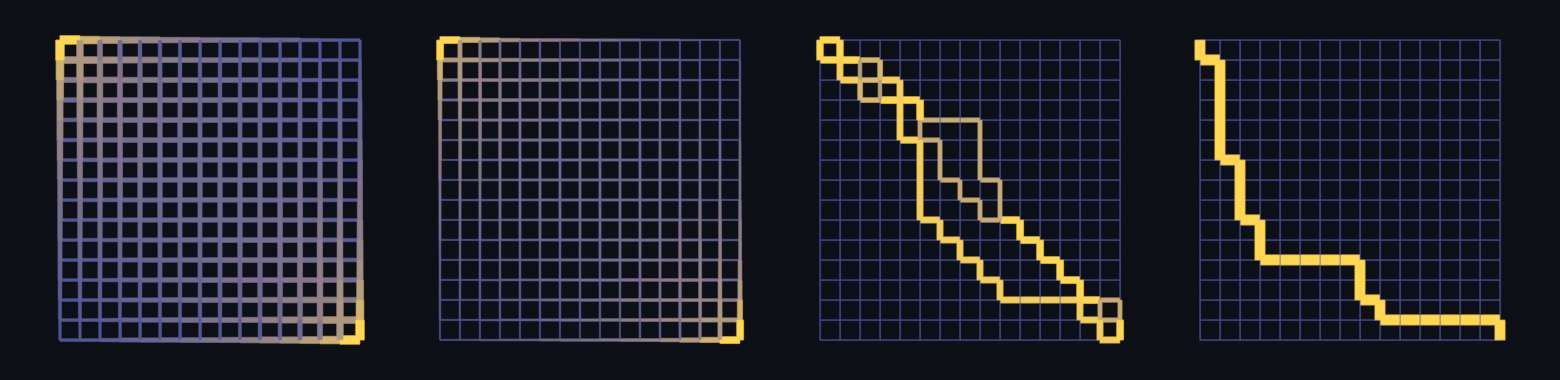
\includegraphics[width=\textwidth]{figs/fig19_networks.png}
\caption{Adapted networks on a $16\times16$ grid with the source at the upper left and the sink at the lower right, for $\mu=0.5$, $1.0$, $1.2$ and $1.5$ from left to right, seed $0$. Edge width is $0.06+0.9D$ and colour shows the flow from $0$ (blue) to $0.5$ (yellow), by one material reading a custom property.}
\end{figure}

\section{What These Experiments Do Not Show}

All results are for one grid size, $16\times16$, one source and sink position, one noise level, and one integration step, with ten seeds per exponent and $1500$ steps. The exponent values are a coarse sample, and the location of the transition between $\mu=1.0$ and $\mu=1.5$ was not found more finely than the row for $1.2$. The $\mu=1.2$ row is nearly but not exactly converged. Nothing was varied in the form of the reinforcement function, in the grid, or in the conductance floor of $0.01$ that decides which edges count as kept, and the cycle count depends on that floor. The statement that the rule is used for the slime mould is recalled from reading. Nothing here shows that any biological or engineered network follows the rule, nor that its parameters correspond to measured quantities, and the total conductance and the dissipation are quantities of the model and not of a material. The Blender scene shows that the solver's state survives translation into geometry and back. It is not a check of the model.

\begin{exercise}[19.1: Locate the transition]
Run $\mu=1.05$, $1.1$, $1.15$, $1.25$, $1.3$ and $1.4$ on ten seeds, with enough steps that the largest rate of change falls below $10^{-8}$, and report the number of kept edges for each. State the smallest exponent at which every seed gave a single path.
\end{exercise}

\begin{exercise}[19.2: Another source]
Move the sink from the opposite corner to the middle of the far edge and repeat the runs at $\mu=0.8$, $1.0$ and $1.5$. State how the length of the final path and the number of loops depend on the geometry, and compare the lengths with the shortest route.
\end{exercise}

\begin{exercise}[19.3: A budget]
After each adaptation step, rescale the conductances so that their sum stays at $30$. Repeat the exponent sweep and report whether the dissipation is now minimised near any exponent. State what the constraint changes about the comparison in Section 19.3.
\end{exercise}

\begin{exercise}[19.4: Read it from the scene]
Delete one edge object from the saved scene of Section 19.5 and re-solve from the remaining geometry. Report which of the checks of that section detect the change, and what the balance residual shows.
\end{exercise}
